\documentclass[preprint]{../PGAS10/sigplanconf}

% The following \documentclass options may be useful:
%
% 10pt          To set in 10-point type instead of 9-point.
% 11pt          To set in 11-point type instead of 9-point.
% authoryear    To obtain author/year citation style instead of numeric.

\usepackage{amsmath}
\usepackage[dvips]{graphicx}
\DeclareGraphicsExtensions{.eps, .ps}
\usepackage[caption=false,font=footnotesize]{subfig}
\usepackage{url}
\usepackage{listings}
\lstset{ %
language=Python,                % choose the language of the code
basicstyle=\ttfamily\footnotesize,  % the size of the fonts that are used for the code
keywordstyle=\bfseries,
frame=single,	                % adds a frame around the code
tabsize=4,   	                % sets default tabsize to 2 spaces
captionpos=b,                   % sets the caption-position to bottom
breaklines=true,                % sets automatic line breaking
breakatwhitespace=false,        % sets if automatic breaks should only happen at whitespace
escapeinside={\%*}{*)},          % if you want to add a comment within your code
xleftmargin=5mm,                % indent listing slightly to get line numbers back onto page
xrightmargin=5mm,
numbers=left, numberstyle=\ttfamily\bfseries\footnotesize
}

% correct bad hyphenation here
\hyphenation{Dist-Num-Py}

\begin{document}

\conferenceinfo{PGAS'10}{New York, New York USA.} 
\copyrightyear{2010} 
\copyrightdata{978-1-4503-0461-0/10/10}

%\titlebanner{DistNumPy}        % These are ignored unless
\preprintfooter{DistNumPy}   % 'preprint' option specified.

\title{Numerical Python for Scalable Architectures}

\authorinfo{Mads Ruben Burgdorff Kristensen \\ Brian Vinter}
           {eScience Centre\\ University of Copenhagen\\ Denmark}
           {madsbk@diku.dk/vinter@diku.dk}

\maketitle

\begin{abstract}

\end{abstract}

\section{Introduction}
In this paper we introduce generic latency hiding for Distributed Numerical Python (DistNumPy)\cite{distnumpy09}, which is a library for doing numerical computation in Python that targets scalable distributed memory architectures. DistNumPy extends the NumPy module\cite{numpy}, which is popular for scientific programming. Replacing NumPy with DistNumPy enables the user to write sequential Python programs that seamlessly utilize distributed memory architectures.

Communication latency hiding is well known technique to improve the performance and scalability of communication bound problems. We define latency hiding informally as in \cite{Strumpen94latencyhiding} -- ``a technique to increase processor utilization by transferring data via the network while continuing with the computation at the same time''.

There exist a lot of methods to implement latency hiding and most of them are tailored to a particular problem. The current method used in DistNumPy to hide the communication latency is also tailored to a particular problem -- namely an element-by-element computation on distributed arrays that uses identical distribution schemes. However, a broad range of DistNumPy programs make use of distributed arrays that do not share identical distribution schemes. In this paper we therefore introduce a generic method for latency hiding that is not tailored to any particular problem.

\subsection{Motivation}
\subsection{Related work}

\section{Distributed Numerical Python}
The programming language Python combined with the numerical library NumPy\cite{numpy} has become a popular numerical framework amongst researchers. It offers a high level programming language to implement new algorithms that support a broad range of high-level operations directly on vectors and matrices.

The idea in NumPy is to provide a numerical extension to the Python language that enables the Python language to be both high productive and high performing. NumPy provides not only an API to standardized numerical solvers, but a possibility to develop new numerical solvers that are both implemented and efficiently executed in Python, much like the idea behind the MATLAB\cite{guide1998mathworks} framework. 

DistNumPy is a new version of NumPy that parallelizes array operations in a manner completely transparent to the user -- from the perspective of the user, the difference between NumPy and DistNumPy is minimal. DistNumPy can use multiple processors through the communication library Message Passing Interface (MPI)\cite{mpi}. However, DistNumPy do not use the traditional SPMD parallel programming model because it requires the user to differentiate between the MPI-processes. Instead the MPI communication in DistNumPy is fully transparent and the user needs no knowledge of MPI or any parallel programming model. 
The only difference in the API of NumPy and DistNumPy is the array creation routines. DistNumPy allow both distributed and non-distributed arrays to co-exist thus the user must specify, as an optional parameter, if the array should be distributed. The following illustrates the only difference between the creation of a standard array and a distributed array:
\lstset{frame=none, xleftmargin=0mm, numbers=none}
\begin{lstlisting}
#Non-Distributed
A = numpy.array([1,2,3])
#Distributed
B = numpy.array([1,2,3], dist=True)
\end{lstlisting}
\lstset{frame=single, xleftmargin=5mm, numbers=left}


\section{Data Layout}
The data layout used in DistNumPy consists of three levels (Fig. \ref{fig:view_block}). The first level is the base-block level, in which a base-block map directly into one block of memory located on one node. The memory block is not necessarily contiguous but only one MPI-process has exclusive access to the block. A base-block is the basic building block in the distribution scheme used when distributing DistNumPy arrays across multiple MPI-processes. The distribution scheme used in DistNumPy is the N-Dimensional Block Cyclic Distribution\cite{distnumpy09} inspired by High Performance Fortran\cite{Loveman93}. 

The second level is the view-block level, which is an abstraction level above the base-block level. A view-block represents a basic block of an array-view, which means that a view-block is a contiguous block of array elements from the perspective of the user. A view-block can span over multiple base-blocks and consequently also over multiple MPI-processes. For a MPI-process to access a whole view-block it will have to fetch data from possible remote MPI-processes and put the pieces together before accessing the block. To avoid this process, which may require some internal memory copying, we divide view-blocks into sub-view-block.

Sub-view-block is the third block level and is simply a block of data that is a part of a view-block but is located on only one MPI-process. The general idea is that all array operation is translated into a number of sub-view-block operations.

We will define a \emph{aligned array} as an array that have a direct contiguous mapping through the block hierarchy. That is, a distributed array in which the base-blocks, view-blocks and sub-view-blocks are identical. A \emph{non-aligned array} is then a distributed array without this property.

\begin{figure}
 \centering
 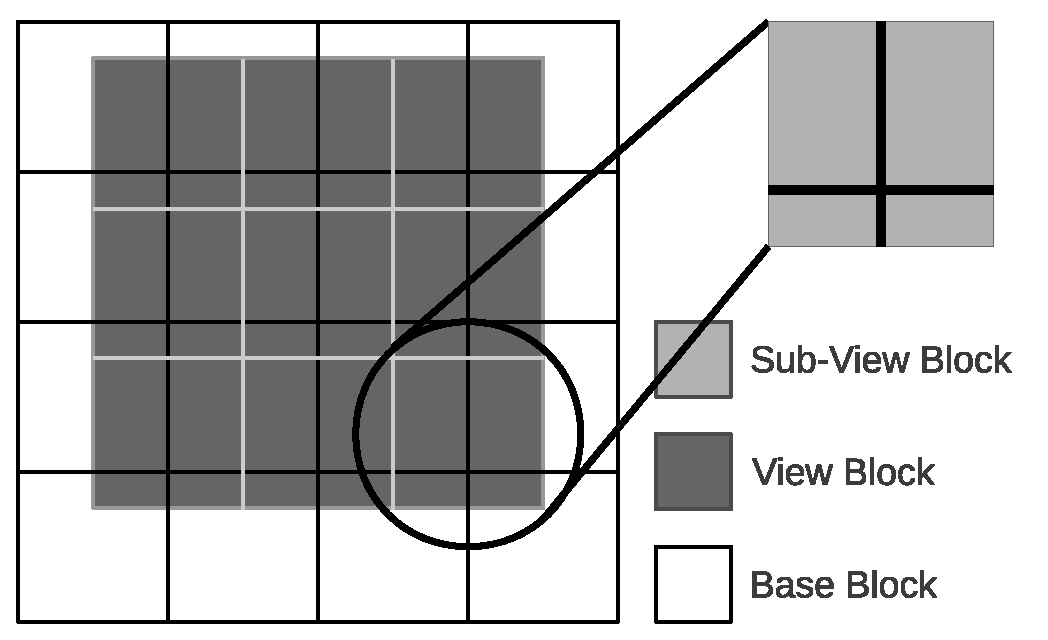
\includegraphics[width=150px]{gfx/view_blocks}
 \caption{An illustration of the block hierarchy used in representing a 2D distributed array. The array is divided into three block-types: Base, View and Sub-View-blocks. The 16 base-blocks make up the base-array, which may be distributed between multiple MPI-processes. The 9 view-blocks make up a view of the base-array and represent the elements that are visible to the user. Each view-block is furthermore divided into four sub-view-blocks, which are the basic block of elements and is always located on one MPI-process.}
 \label{fig:view_block}
\end{figure}


\section{Universal Function}
An important mechanism in DistNumPy is a concept called Universal function. A universal function (ufunc) is a function that operates on all elements in an array-view independently. That is, an ufunc is a vectorized wrapper for a function that takes a fixed number of scalar inputs and produces a fixed number of scalar outputs. E.g. addition is an ufunc that takes three array-views as argument: two input arrays and one output array; and for each element the two input arrays are added together and the result is written to the output array. Using ufunc can result in a significant performance boost compared to native Python because the computation-loop is implemented in C and is executed in parallel.

Performing an ufunc operation on a whole array-view is semantically equivalent to performing the ufunc operation on each array-view block individually. It is this property that makes it possible to perform a distributed ufunc operation in parallel. 

A distributed ufunc operation consists of four steps: 
\begin{enumerate}
\item Each MPI-process determents which view-blocks of the ufunc operation that is should compute. This is strictly based on the distributed of the output array-view. 
\item All MPI-processes exchange array elements in such a manner that all MPI-processes can perform its computation locally. 
\item All MPI-processes performs its local computation.
\item All MPI-processes sends the written array elements back to the original locations.
\end{enumerate}



\section{Latency Hiding}
\begin{figure}
 \centering
 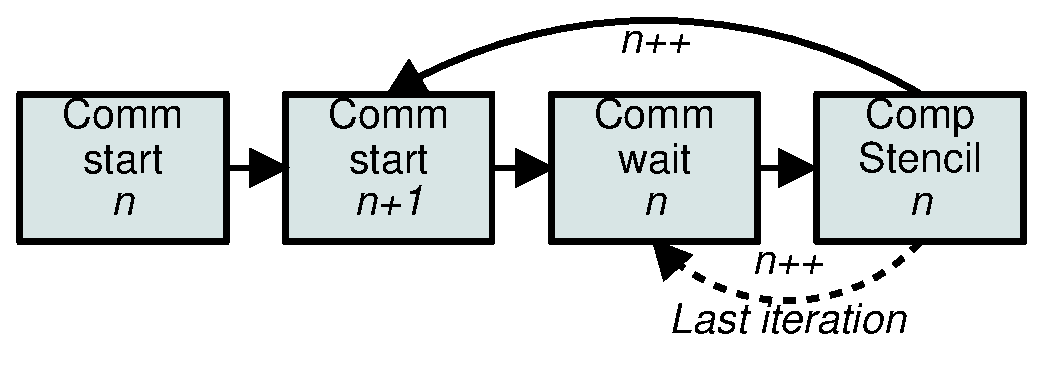
\includegraphics[width=200px]{gfx/double_buffering}
 \caption{Flow diagram illustrating double buffering. The $n$'th iteration is expressed with a $n$ and Comm and Comp represents communication and computation, respectively. $n$++ is an iteration to $n$'s successor.}
 \label{fig:double_buffering}
\end{figure}

The standard approach to hide communication latency behind computation in message-passing is a technique known as double buffering. The implementation of double buffering is straightforward when operating on a set of data block that all have identical sizes. The communication of one data block is overlapped with the computation of another already communicated data block (Fig. \ref{fig:double_buffering}) and since the sizes of all the data blocks are identical all iterations are also identical.

The straightforward double buffering approach is used in the current version of DistNumPy. It works very well for ufuncs that operates on aligned arrays because it translates into complete communication and computation view-block operations. Therefore is there no need to introduce latency hiding inside a view-block because the whole view-block is located on a single MPI-process. This is not the case for ufuncs that operates on non-aligned arrays where view-blocks are located on multiple MPI-processes. I order to achieve good performance some latency hiding inside view-blocks must be introduced. For example the computation of a view-block in figure \ref{fig:view_block} can make use of latency hiding by first initiate the communication of the three non-local sub-view-blocks, then compute the local sub-view-block and finally compute the three communicated sub-view-blocks. 

What is needed is a generic approach that, based on the executing program, schedules the communication and computation in an overlapping pattern. Since Python is an interpreted interactive programming language it is not possible to schedule communication and computation operation at compile time. Instead some kind of look-ahead technique is required to determine the communication and computation operations used in the program at runtime. 


\section{Lazy Evaluation}
To make it possible for a scheduler to schedule communication behind computation operations we introduce Lazy Evaluation. During the execution of a DistNumPy program all MPI-processes records the requested array operations rather than applying them immediately. The operations are maintained in a convenient data structure and at a later point all MPI-processes perform the operations. The idea is that by having a bunch of operations to carry out it may be possible to schedule communication and computation operations that have no mutual dependencies in parallel.

We will only introduce lazy evaluation for Python operations that involve DistNumPy arrays. Python operations that do not include DistNumPy arrays will simple be executed by the Python interpreter immediately. Thus DistNumPy array operations that involve program branches will also have to be executed immediately because a branch may lead to non-DistNumPy operations. What this boils down to is: whenever we encounter a branch all previously recorded operations must be executed. This mechanism of executing all previously recorded operation we will call an \emph{operation flush}. The two only other conditions that can trigger an operation flush is when the number of recorded operations reaches a user-defined threshold or when the Python interpreter reaches the end of the program. Furthermore only complete flushes are used.


\subsection{The Dependency System}
The main challenge when introducing Lazy Evaluation is to implement a dependency system that schedules operations in a performance efficient manner while the overhead is kept at an acceptable level.

The partial order of operations imposed by operational dependencies is normally represented by a directed acyclic graph (DAG)\cite{AhSeUl86}. The nodes of the DAG represent operations and the edges represent the dependencies between the operations. E.g. a DAG with two nodes $A$ and $B$ and an edge from $A$ to $B$ means that $A$ must be executed before $B$ to preserve correctness of the overall program. 

Our first lazy evaluation approach makes use of a DAG to contain all recorded operations. A small Python program that makes use of DistNumPy and the corresponding DAG is illustrated in figure 3 and 4. Beside the DAG our dependency system also consist of a \emph{ready queue}, which is a queue of recorded operations that do not have any dependencies. The ready queue makes it possible in to find operations that are ready to be executed in the time complexity of $O(1)$.


\begin{figure}
\begin{lstlisting}
import numpy as np
base = np.array([1,2,3,4,5],dist=True)
A = base[:2]  #A = [1,2]
B = base[3:]  #B = [4,5]
T = A + B     #T = [5,7]
T = T * B	  #T = [20,35]
print T
\end{lstlisting}
 \caption{This is an example of a small Python program that makes use of DistNumPy.}
 \label{lst:code_eg}
\end{figure}

\begin{figure}
 \centering
 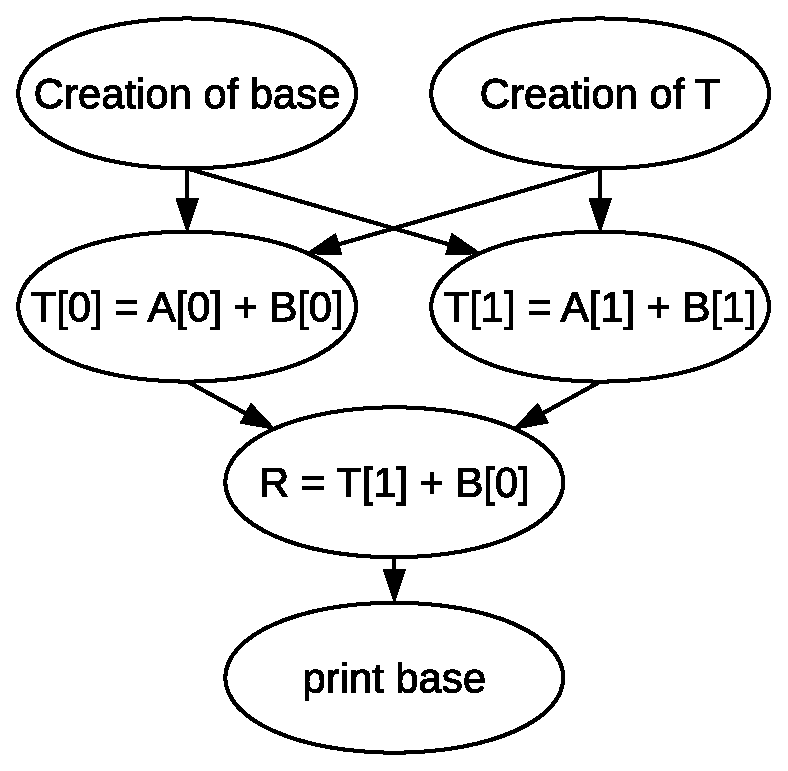
\includegraphics[width=120px]{gfx/dag}
 \caption{This figure illustrates a directed acyclic graph that represents the operational dependencies in figure \ref{lst:code_eg}. The size of the view-blocks is one and the number inside brackets is a reference to a view-block.}
 \label{fig:DAG}
\end{figure}


\subsubsection{Operation Insertion}
The recording of an operation is basically an insertion of new node into the DAG. A straightforward insertion approach is simple to compare the new node with all nodes already located in the DAG and possible add new edges between conflicts. The time complexity of insertion is then $O(n)$ where $n$ is the number of operation in the DAG and the construction of the complete DAG is $O(n^2)$.

%In worse case this approach is optimal because the longest path through the DAG is always $n$. However, we have introduced some heuristics to speed up the common case. 

\subsubsection{Operation Flush}
The main goal when performing an operation flush is to overlap communication with computation. Our approach to achieve this goal is to initiate communication at the earliest point in time and only do computation when all communication has been initiated. Furthermore, to make sure that there is progress in the MPI layer we check for finished communication in between multiple computation operations. The following is the flow of our operation flush algorithm:
\begin{enumerate}
\item Initiate all communication operation in the ready queue.
\item Check in a non-blocking manner if some communication operations have finished and remove possible finished communication operations from the ready queue and the DAG. Furthermore, register operations that now have no dependencies into the ready queue.
\item If there is only computation operations in the ready queue execute one of them and remove it from the ready queue and the DAG.
\item Go back to step one if there is any operation left in the ready queue, else we are finished.
\end{enumerate}
The algorithm maintains the folowing three invariants:
\begin{enumerate}
\item All operations that are ready are located in the ready queue.
\item We only start the execution of a computation node when there is no communication node in the ready queue.
\item We only wait for communication when the ready queue have no computation nodes.
\end{enumerate}



\subsubsection{Dependency Heuristic}
Experiments with lazy evaluation using the dependency DAG shows that the overhead associated with the creation of the DAG is very time consuming and becomes the dominating performance factor. This cannot be helped in the worse case, but we have introduced a heuristic to speed up the common case. 

The heuristic is based on the observation that normally a computation is evenly spread out between all sub-view-blocks in the involved arrays and that it is only possible to have conflict between sub-view-blocks that are part of the same base-block. The idea is that instead of having one DAG only, we introduce a DAG for each base-block -- the assumption is that in the common case the size of each DAG will be dramatically reduced. Actually we expect the size of the DAGs to be at a level where it makes most sense to use a linked list rather than in a full-blown DAG.


\begin{figure}
 \centering
 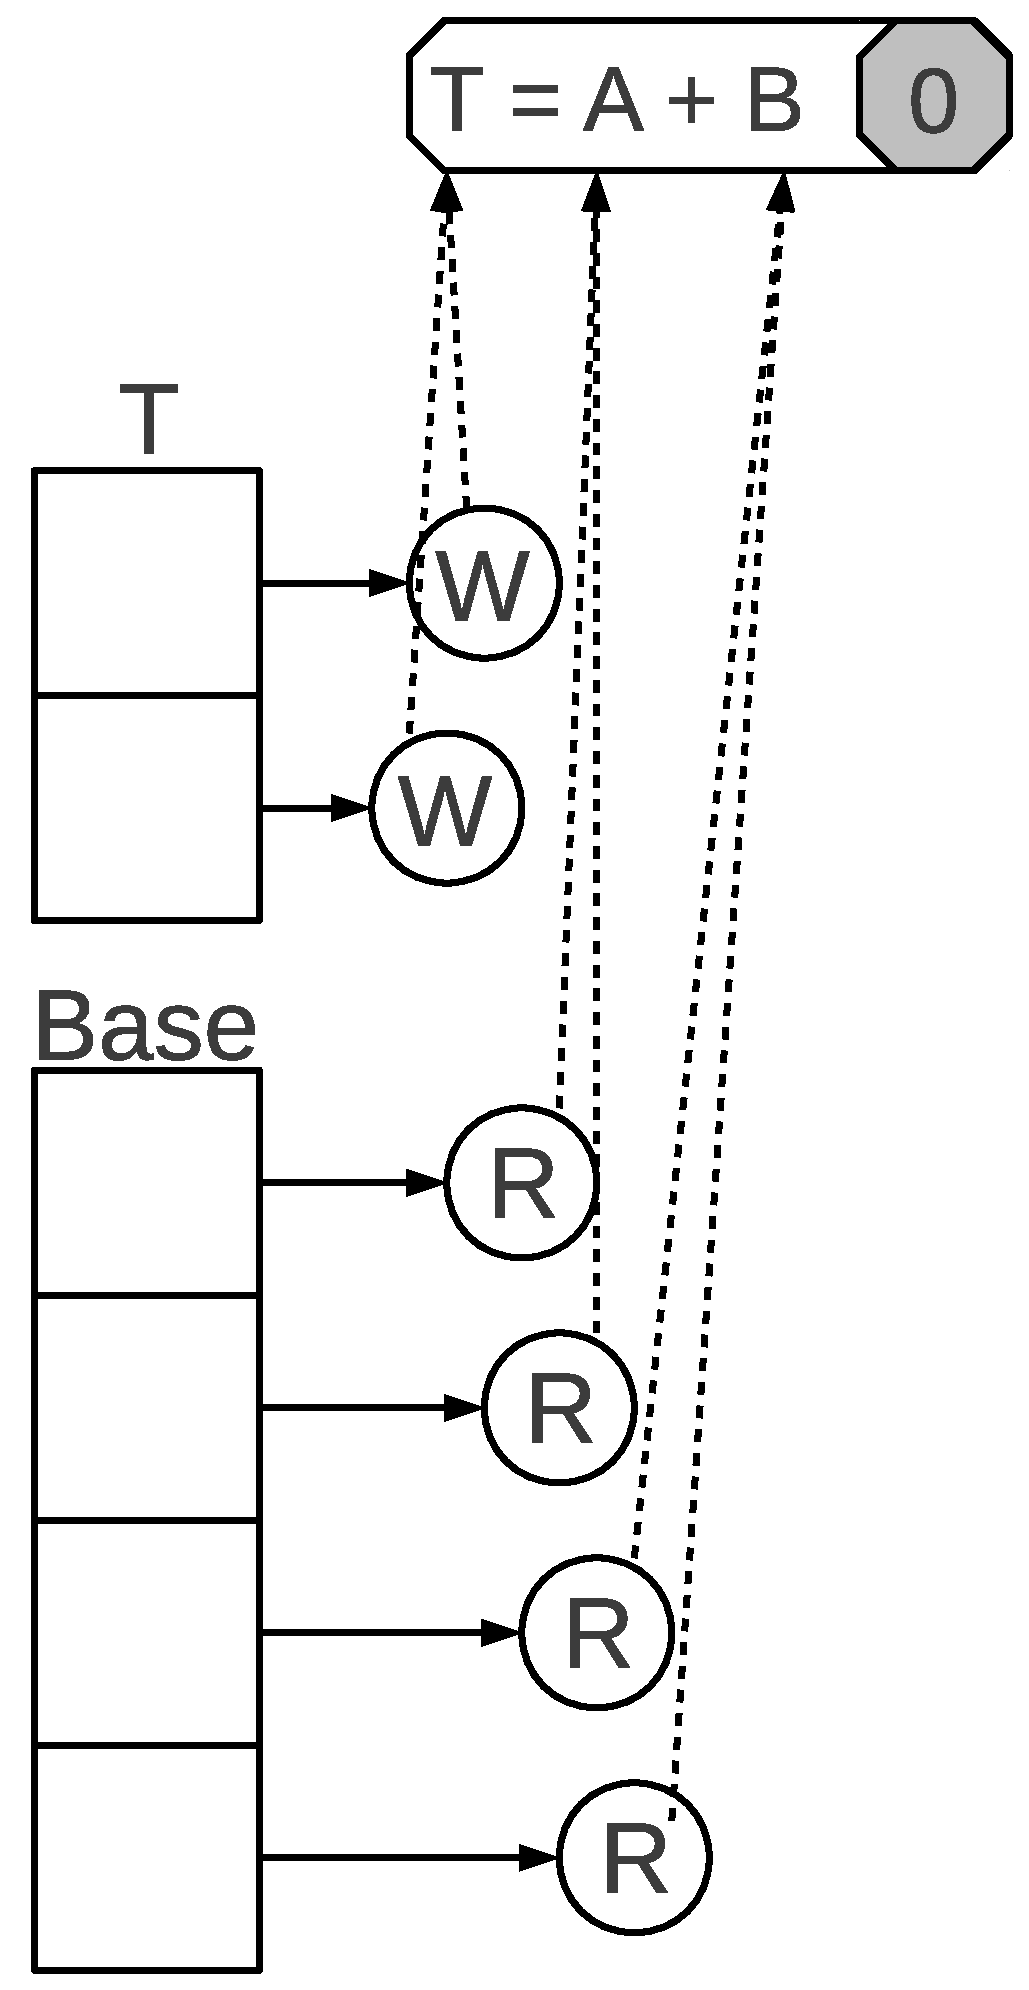
\includegraphics[width=50px]{gfx/dependency_system}
 \caption{dependency system}
 \label{fig:dependency_system}
\end{figure}









%Lazy evaluation on these data blocks are managed through a simple dependency list for each block. When a NumPy operation is issued it is split across the sub-view blocks that are involved in the operation. For each such operation on a sub-view block a set of tasks are created, one for each combined set of data-blocks to sub-view blocks. Dependencies are then added to the dependency-list of each data-block that is involved, each dependency link back to the individual tasks. When the number of dependencies on a task reached zero the task may be moved to the ready-queue. But before this is done we traverse the dependency list and include any other task that can be merged into the ready task, given that they could execute in parallel with the task or could execute given the task was done, when two tasks are merged into one, the remaining list is traversed under the same rules but for the merged task.


\subsection{Ufunc Operation List}




\section{Examples}


\section{Experiments}


\section{Future work}


\section{Conclusions}


\bibliographystyle{IEEEtran}
\bibliography{/home/madsbk/repos/priv/diku/phd/paper_archive/main}

\end{document}